\section{Dataset} \label{sec:dataset}

\textbf{(*VP* Sposterei questa sezione nel prossimo cap, che potresti intitolare Dataset and Data Preprocessing. )}
The dataset at our disposal describes a period of almost two years
(from 02-02-2022 to 16-06-2023) and comes from a 978 kW photovoltaic
plant located in the province of Bari. It consists of 3 inverters,
27 field panels, 1 meter, 1 solarimeter, 2 interface protections
and 1 \textquote{system} device in which data from Solargis are stored.
The dataset is organized into files, one for each type of device,
representing each individual day, and the data is aggregated
every 5 minutes. Each row contains a reference to the device
it belongs to (\verb|deviceName| and \verb|deviceId|).


%Il dataset a nostra disposizione descrive un periodo di quasi due anni (dal
%02/02/2022 al 16/06/2023) ed è proveniente da un impianto fotovoltaico da 978 kW
%situato nella provincia di Bari. È composto da
%3 inverter, 27 quadri di campo, 1 contatore, 1 solarimetro, 2 protezioni
%interfaccia e 1 dispositivo \textquote{impianto} nel quale vengono immagazzinati
%i dati provenienti da Solargis. Il dataset è organizzato in file, uno per
%tipologia di dispositivo, che
%rappresentano la singola giornata e i dati sono aggregati a 5 minuti ed ogni
%riga riporta il riferimento al
%dispositivo di appartenenza (\verb|deviceName| e \verb|deviceId|).

\begin{table}[H]
	\begin{center}
		\begin{tabular}[c]{l}
			\hline
			\textbf{File Name}                                  \\
			\hline
			\verb|2022_02_02_Rofilo_NP00003174_inverter.csv|    \\
			\verb|2022_02_02_Rofilo_NP00003174_meteorology.csv| \\
			\verb|2022_02_02_Rofilo_NP00003174_meter.csv|       \\
			\verb|2022_02_02_Rofilo_NP00003174_other.csv|       \\
			\verb|2022_02_02_Rofilo_NP00003174_plantDevice.csv| \\
			\verb|2022_02_02_Rofilo_NP00003174_stringbox.csv|   \\
			\verb|2022_02_03_Rofilo_NP00003174_inverter.csv|    \\
			\verb|2022_02_03_Rofilo_NP00003174_meteorology.csv| \\
			\verb|2022_02_03_Rofilo_NP00003174_meter.csv|       \\
			\verb|2022_02_03_Rofilo_NP00003174_other.csv|       \\
			\verb|2022_02_03_Rofilo_NP00003174_plantDevice.csv| \\
			\verb|2022_02_03_Rofilo_NP00003174_stringbox.csv|   \\
			$\ldots$                                            \\
			\hline
		\end{tabular}
	\end{center}
	\caption{Some files from our dataset.}\label{tab:datasunto}
\end{table}

\begin{table}[H]
	\begin{center}
		\begin{tabular}[c]{l|l|l|l|l|l}
			\hline
			\multicolumn{1}{c|}{\textbf{timestamp}}        &
			\multicolumn{1}{c|}{\textbf{serial}}           &
			\multicolumn{1}{c|}{\textbf{$\ldots$}}         &
			\multicolumn{1}{c|}{\textbf{TotalEnergy(kWh)}} &
			\multicolumn{1}{c|}{\textbf{Frequency(Hz)}}    &
			\multicolumn{1}{c}{\textbf{deviceid}}            \\
			\hline
			2022-10-23 04:30:00                            &
			INV01                                          &
			$\ldots$                                       &
			357196.88                                      &
			50.06                                          &
			83204                                            \\

			2022-10-23 04:35:00                            &
			INV01                                          &
			$\ldots$                                       &
			357196.88                                      &
			50.06                                          &
			83204                                            \\

			%			01/02/2023 00:15                               &
			%			INV01                                          &
			%			$\ldots$                                       &
			%			431324.36                                      &
			%			49.88                                          &
			%			83204                                            \\

			$\ldots$                                       &
			$\ldots$                                       &
			$\ldots$                                       &
			$\ldots$                                       &
			$\ldots$                                       &
			$\ldots$                                         \\
			2022-10-23 13:00:00                            &
			INV01                                          &
			$\ldots$                                       &
			357921.16                                      &
			49.95                                          &
			83204                                            \\
			2022-10-23 13:05:00                            &
			INV01                                          &
			$\ldots$                                       &
			357935.24                                      &
			49.95                                          &
			83204                                            \\
			%			01/02/2023 12:10                               &
			%			INV01                                          &
			%			$\ldots$                                       &
			%			431324.36                                      &
			%			49.88                                          &
			%			83204                                            \\

			$\ldots$                                       &
			$\ldots$                                       &
			$\ldots$                                       &
			$\ldots$                                       &
			$\ldots$                                       &
			$\ldots$                                         \\
			01/02/2023 23:45                               &
			INV01                                          &
			$\ldots$                                       &
			431324.36                                      &
			49.88                                          &
			83204                                            \\
			01/02/2023 23:50                               &
			INV01                                          &
			$\ldots$                                       &
			431324.36                                      &
			49.88                                          &
			83204                                            \\
			%			01/02/2023 23:55                               &
			%			INV01                                          &
			%			$\ldots$                                       &
			%			431324.36                                      &
			%			49.88                                          &
			%			83204                                            \\
			\hline
		\end{tabular}
		\caption{Some lines from an Inverter file.}\label{tab:invsunto}
	\end{center}
\end{table}

\subsection{Inverter}
Inside the files related to the inverters, we can find data such as
the processor's operating temperature
(\verb|InternalTemperature|), various Alternating and Direct currents
produced (\verb|CurrentAC| and \verb|CurrentDC|), Delivered Power,
total energy produced by the individual inverter and other status
and control bits that indicate various stages of the inverter's
life (boot, reset, ready, etc.).

Down below a table with all the available features:


%Nei file relativi agli inverter posiamo trovare dati come la temperatura di
%funzionamento del processore (\verb|InternalTemperature|), le varie correnti
%alternate e continue prodotte (\verb|CurrentAC| e \verb|CurrentDC|), la Potenza Erogata, l'energia totale prodotta dal singolo inverter più altri
%bit di stato e controllo che mostrano le varie fasi di vita dell'inverter (boot, reset, ready, ecc.).\\
%Di seguito una tabella con tutte le features a disposizione:
%Un inverter in un impianto fotovoltaico è un componente fondamentale che svolge
%una funzione vitale: converte l'energia elettrica prodotta dai pannelli solari,
%che è in corrente continua (DC), in energia elettrica utilizzabile in corrente
%alternata (AC). Questa conversione è cruciale perché la maggior parte delle
%apparecchiature elettriche domestiche e delle reti di distribuzione elettrica
%utilizzano corrente alternata per funzionare.
%Regolano la
%tensione e la frequenza della corrente alternata prodotta per garantire che
%siano conformi agli standard di rete elettrica locale. Questo è importante
%per evitare danni agli apparecchi elettrici e per garantire
%l'interoperabilità con la rete elettrica.
%Sono spesso dotati di
%tecnologie avanzate come il "Maximum Power Point Tracking" (MPPT) che
%ottimizzano costantemente la produzione di energia solare. Questo significa
%che l'inverter regola la tensione in ingresso dai pannelli solari per
%ottenere la massima potenza possibile in base alle condizioni di luce solare
%in tempo reale.
%Le feature che caratterizzano il nostro impianto sono riassunte dalla seguente
%tabella:

\begin{table}[H]
	\begin{center}
		\begin{tabular}[c]{l|l|l}
			\hline
			\multicolumn{1}{c|}{\textbf{Name}}        &
			\multicolumn{1}{c|}{\textbf{Unit Symbol}} &
			\multicolumn{1}{c}{\textbf{Description}}                                     \\
			\hline
			CommunicationCode                         & -   & Communication Code         \\
			Failure 3                                 & -   & Active Alarm               \\
			Failure 4                                 & -   & Isolation Alarm            \\
			CurrentDC                                 & A   & Photovoltaic field Current \\
			CurrentAC                                 & A   & Network Current            \\
			CurrentAC Phase1                          & A   & Line RMS Current Phase R   \\
			CurrentAC Phase2                          & A   & Line RMS Current Phase S   \\
			CurrentAC Phase3                          & A   & Line RMS Current Phase T   \\
			TotalEnergy                               & kWh & Active Energy Delivered    \\
			Frequency                                 & Hz  & Network Frequency          \\
			PowerAC Phase1                            & kW  & Line PA Phase R            \\
			PowerAC Phase2                            & kW  & Line PA Phase S            \\
			PowerAC Phase3                            & kW  & Line PA Phase T            \\
			PowerAC                                   & kW  & Delivered PA               \\
			PowerDC                                   & kW  & Photovoltaic field Power   \\
			Status                                    & -   & Inverter State             \\
			Failure                                   & -   & Network docking PLL State  \\
			Failure 2                                 & -   & Network State 1            \\
			Failure 1                                 & -   & Network State  2           \\
			InternalTemperature                       & C   & CPU Temp.                  \\
			HeatSinkTemperature                       & C   & IGBT Temp.                 \\
			VoltageDC                                 & V   & Photovoltaic field Voltage \\
			VoltageAC                                 & V   & Network Voltage            \\
			VoltageAC Phase1                          & V   & Line RMS Voltage Phase R   \\
			VoltageAC Phase2                          & V   & Line RMS Voltage Phase S   \\
			VoltageAC Phase3                          & V   & Line RMS Voltage Phase T   \\
			\hline
		\end{tabular}
		\caption{All available features from an \texttt{inverter} file.}\label{tab:invfeatures}
	\end{center}
\end{table}

\begin{figure}[H]
	\centering
	\begin{subfigure}[t]{0.45\textwidth}
		\centering
		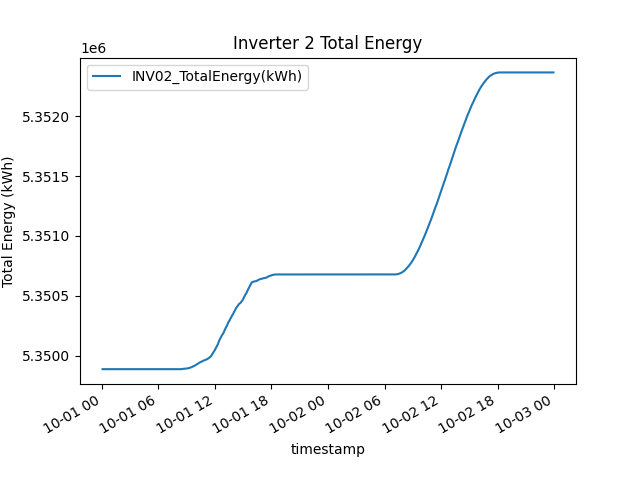
\includegraphics[width=\textwidth, keepaspectratio]{chapters/1_introduction/imgs/inv2totenergy.png}
		\caption{Inverter 2 Total Energy plot.}
		\label{fig:inv02totenergy}
	\end{subfigure}
	\hspace{0.5cm}
	\begin{subfigure}[t]{0.45\textwidth}
		\centering
		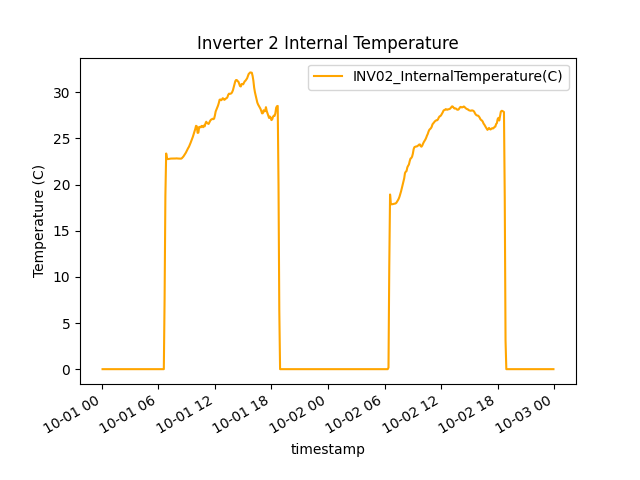
\includegraphics[width=\textwidth, keepaspectratio]{chapters/1_introduction/imgs/inv2temperature.png}
		\caption{Inverter 2 CPU Temperature plot.}
		\label{fig:inv02temp}
	\end{subfigure}\\

	\begin{subfigure}[t]{0.45\textwidth}
		\centering
		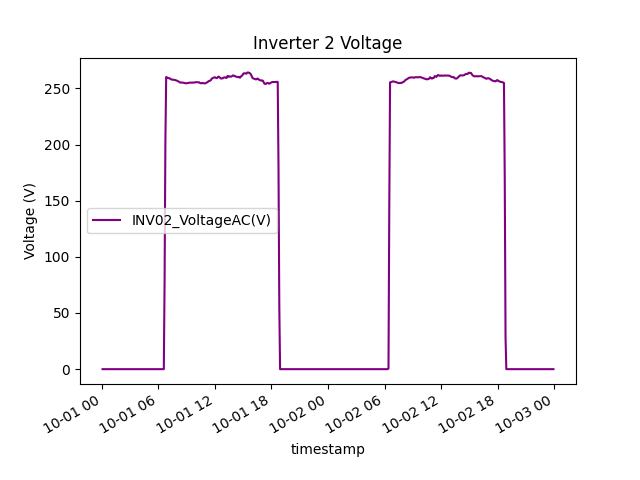
\includegraphics[width=\textwidth, keepaspectratio]{chapters/1_introduction/imgs/inv2voltage.png}
		\caption{Inverter 2 Voltage AC plot.}
		\label{fig:inv02volt}
	\end{subfigure}
	\hspace{0.5cm}
	\begin{subfigure}[t]{0.45\textwidth}
		\centering
		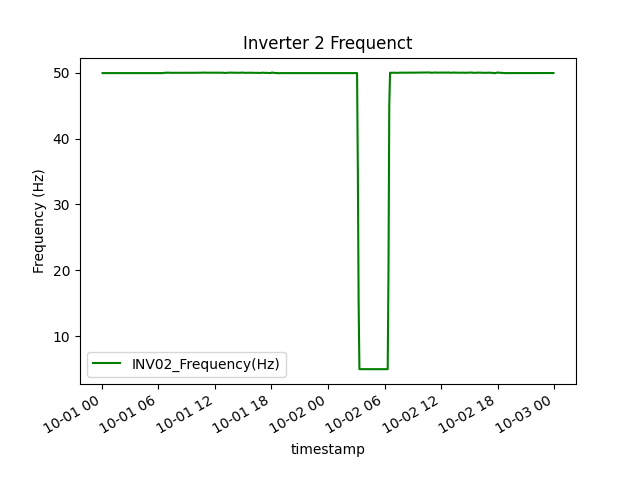
\includegraphics[width=\textwidth, keepaspectratio]{chapters/1_introduction/imgs/inv2freq.png}
		\caption{Inverter 2 Frequency plot.}
		\label{fig:inv02freq}
	\end{subfigure}
\end{figure}


%\subsection{StringBox}
%Le stringbox in un impianto fotovoltaico sono contenitori elettrici progettati
%per ospitare e proteggere una serie (o stringa) di pannelli solari collegati in
%serie. Questi dispositivi svolgono diverse funzioni importanti:
%
%\begin{itemize}
%	\item Protezione: Le stringbox includono dispositivi di protezione come interruttori
%	      automatici o fusibili che prevengono cortocircuiti e sovraccarichi nel circuito
%	      fotovoltaico.
%	\item Connettori: Forniscono connettori sicuri per collegare i cavi provenienti dai
%	      pannelli solari alla stringa di cavi principale dell'impianto.
%	\item Monitoraggio: Alcune stringbox sono dotate di sistemi di monitoraggio che
%	      consentono di rilevare prestazioni o guasti dei pannelli solari all'interno
%	      della stringa.
%	\item Isolamento: Possono anche includere dispositivi di isolamento che consentono di
%	      interrompere l'alimentazione elettrica verso la stringa di pannelli solari per
%	      scopi di manutenzione o sicurezza.
%\end{itemize}

\subsection{Junction Box}
In the files related to the Junction Box or Combiner Box, we find data that describes
the current production of the various strings they are connected to (\verb|CurrentString1-7|,
in general, each Junction Box manages 7 strings), some temperatures (such as
\verb|ModuleTemperature|), and some control bits to check proper operation.


%Nei file relativi alle Junction Box o Combiner Box, troviamo dati che
%descrivono la produzione di corrente delle varie stringhe a cui sono collegati (\verb|CurrentString1-7|, in generale ogni Junction Box gestisce 7 stringhe), alcune temperature (come \verb|ModuleTemerature|) e alcuni bit di controllo per verificare il corretto funzionamento.

\begin{table}[H]
	\begin{center}
		\begin{tabular}[c]{l|l|l}
			\hline
			\multicolumn{1}{c|}{\textbf{Name}}        &
			\multicolumn{1}{c|}{\textbf{Unit Symbol}} &
			\multicolumn{1}{c}{\textbf{Description}}                                             \\
			\hline
			CommunicationCode                         & -              & Communication Code      \\
			Failure                                   & -              & Strings Alarm           \\
			CurrentString1                            & A              & Current I1              \\
			CurrentString2                            & A              & Current I2              \\
			CurrentString3                            & A              & Current I3              \\
			CurrentString4                            & A              & Current  I4             \\
			CurrentString5                            & A              & Current I5              \\
			CurrentString6                            & A              & Current I6              \\
			CurrentString7                            & A              & Current I7              \\
			AverageStringCurrent                      & A              & Average Current         \\
			Irradiance                                & $\text{W/m}^2$ & Modules Irradiation     \\
			Failure 1                                 & -              & Open Strings            \\
			Failure 2                                 & -              & Not Perform. Strings    \\
			EnvironmentTemperature                    & C              & Environment Temperature \\
			ModuleTemperature                         & C              & Modules Temperature     \\
			InternalTemperature                       & C              & Board Temperature       \\
			\hline
		\end{tabular}
		\caption{All available features form a \texttt{stringbox} file.}\label{tab:junctionfeatures}
	\end{center}
\end{table}


\subsection{Solargis} \label{sec:solargis}
Solargis is a company specialized in providing solar data and forecasting services for photovoltaic
installations and solar energy-related projects\cite{solargis}. Their main goal is to provide precise and
reliable information on solar irradiation and solar weather conditions anywhere in the world.
This data is essential for the design, optimization, and management of photovoltaic systems.
Solargis collects and provides detailed data on global, direct, and diffuse solar irradiation at
every geographical location\cite{solargis}. This data allows photovoltaic system developers to assess the
amount of available solar energy in a given area, which is crucial for properly sizing the
system and calculating production forecasts.

%Solargis è una società specializzata nella fornitura di dati e servizi di
%previsione solare per impianti fotovoltaici e progetti legati all'energia
%solare. Il loro principale obiettivo è fornire informazioni precise e affidabili
%sull'irradiazione solare e sulle condizioni meteorologiche solari in qualsiasi
%parte del mondo. Questi dati sono fondamentali per la progettazione,
%l'ottimizzazione e la gestione degli impianti fotovoltaici.
%Solargis raccoglie e fornisce dati dettagliati
%sull'irradiazione solare globale, diretta e diffusa in ogni posizione
%geografica. Questi dati consentono agli sviluppatori di impianti fotovoltaici di
%valutare la quantità di energia solare disponibile in una determinata area, il
%che è fondamentale per dimensionare correttamente l'impianto e calcolare le
%previsioni di produzione.

\begin{table}[H]
	\begin{center}
		\begin{tabular}[c]{l|l|l|l}
			\hline
			\multicolumn{1}{c|}{\textbf{timestamp}}         &
			\multicolumn{1}{c|}{\textbf{$\ldots$}}          &
			\multicolumn{1}{c|}{\textbf{SolargisGHI(W/m2)}} &
			\multicolumn{1}{c}{\textbf{SolargisGTI(W/m2)}}                          \\
			\hline
			2022-08-01 11:40:00                             & $\ldots$ & 896 & 978  \\
			2022-08-01 11:45:00                             & $\ldots$ & 896 & 978  \\
			2022-08-01 11:50:00                             & $\ldots$ & 896 & 978  \\
			2022-08-01 11:55:00                             & $\ldots$ & 914 & 1001 \\
			2022-08-01 12:00:00                             & $\ldots$ & 914 & 1001 \\
			2022-08-01 12:05:00                             & $\ldots$ & 914 & 1001 \\
			2022-08-01 12:10:00                             & $\ldots$ & 928 & 1019 \\
			2022-08-01 12:15:00                             & $\ldots$ & 928 & 1019 \\
			2022-08-01 12:20:00                             & $\ldots$ & 928 & 1019 \\

			\hline
		\end{tabular}
		\caption{Some Solargis data from \texttt{2022\_08\_01\_Rofilo\_NP00003174\_plantDevice.csv} file}\label{tab:solargis}
	\end{center}
\end{table}

\begin{figure}[H]
	\centering
	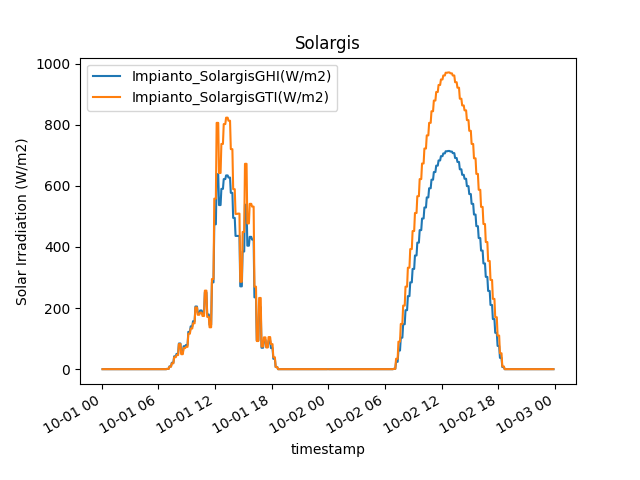
\includegraphics[width=.7\linewidth]{chapters/1_introduction/imgs/solargis.png}
	\caption{Solargis GHI \& GTI plot.}
	\label{fig:solargisplot}
\end{figure}


Solar radiation takes a long journey until it reaches Earth’s surface. So when
modelling solar radiation, various interactions of extra-terrestrial solar
radiation with the Earth’s atmosphere, surface and objects are to be taken into
account\cite{solargis}. The component that is neither reflected nor scattered, and which
directly
reaches the surface, is called direct radiation; this is the component that
produces shadows. The component that is scattered by the atmosphere, and which
reaches the ground is called diffuse radiation. The small part of the radiation
reflected by the surface and reaching an inclined plane is called the reflected
radiation. These three components together create global radiation.

In solar energy applications, the following parameters are commonly used in
practice:

\begin{itemize}
	\item Direct Normal Irradiation/Irradiance (DNI) is the component that is
	      involved in thermal (concentrating solar power, CSP) and photovoltaic
	      concentration
	      technology (concentrated photovoltaic, CPV)\cite{solargis}.
	\item  Global Horizontal
	      Irradiation/Irradiance (GHI) is the sum of direct and diffuse radiation
	      received on a horizontal plane. GHI is a reference radiation for the
	      comparison of climatic zones; it is also essential parameter for
	      calculation of radiation on a tilted plane\cite{solargis}.
	\item Global Tilted Irradiation/Irradiance (GTI), or total
	      radiation received on a surface with defined tilt and azimuth, fixed or
	      sun-tracking. This is the sum of the scattered radiation, direct and
	      reflected. It is a reference for photovoltaic (PV) applications, and
	      can be occasionally affected by shadow\cite{solargis}.
\end{itemize}


\begin{table}[H]
	\begin{center}
		\begin{tabular}[c]{l|l|l}
			\hline
			\multicolumn{1}{c|}{\textbf{Name}}        &
			\multicolumn{1}{c|}{\textbf{Unit Symbol}} &
			\multicolumn{1}{c}{\textbf{Description}}                                                            \\
			\hline
			SolargisGHI                               & $\text{W/m}^2$ & Solargis Global Horizontal Irradiation \\
			SolargisGTI                               & $\text{W/m}^2$ & Solargis Global Tilted Irradiation     \\
			\hline
		\end{tabular}
		\caption{All available features from a \texttt{plantDevice} file.}\label{tab:solargisfeatures}
	\end{center}
\end{table}

\subsection{Meteorology}
In the Meteo files, we can find some environment
temperature and solar irradiance data. Is important to mention that these
features are not as powerful as
weather forecast or Solargis data for the Imputation task.

%Nei file meteo possiamo trovare alcuni dati sulla temperatura
%ambientale e il valore dell'irraggiamento solare. Non risultano
%dati completi come potrebbero essere quelli provenienti da
%previsioni meteo.

\begin{table}[H]
	\begin{center}
		\begin{tabular}[c]{l|l|l}
			\hline
			\multicolumn{1}{c|}{\textbf{Name}}        &
			\multicolumn{1}{c|}{\textbf{Unit Symbol}} &
			\multicolumn{1}{c}{\textbf{Description}}                                        \\
			\hline
			COMMUNICATION\_CODE SOL                   & -              & Communication Code \\
			Irradiance SOL                            & $\text{W/m}^2$ & Irradiance         \\
			Module Temperature HEX SOL                & -              & All Registers      \\
			Module Temperature SOL                    & C              & Module Temperature \\
			\hline
		\end{tabular}
		\caption{All available features from a \texttt{meteo} file.}\label{tab:solargisfeatures}
	\end{center}
\end{table}

\subsection{Meter}
The Meter files contain information about the current injected
into and drawn from the network. It is from here that we get
the values of our target feature \verb|Cont_TotalEnergy(kWh)|.

%I file meter contengono informazioni sulla corrente immessa e prelevata dalla rete.
%\`{E} da qui che andremo a leggere i valori della nostra target feature \verb|Cont_TotalEnergy(kWh)|.

\begin{figure}[H]
	\centering
	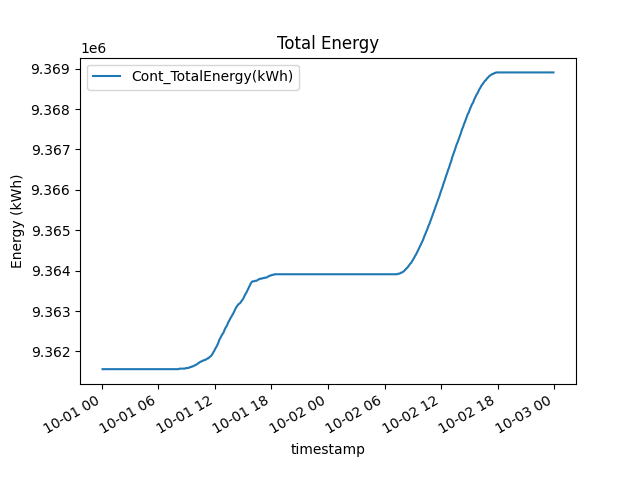
\includegraphics[width=1\linewidth]{chapters/1_introduction/imgs/totalenergy.png}
	\caption{Total Energy plot, our target feature.}
	\label{fig:totenergyplot}
\end{figure}

\begin{table}[H]
	\begin{center}
		\begin{tabular}[c]{l|l|l}
			\hline
			\multicolumn{1}{c|}{\textbf{Name}}        &
			\multicolumn{1}{c|}{\textbf{Unit Symbol}} &
			\multicolumn{1}{c}{\textbf{Description}}                                \\
			\hline
			COMMUNICATION\_CODE Cont                  & -   & Communication Code    \\
			Status Cont                               & -   & Status                \\
			Totale Energia Immessa Cont               & kWh & Total Energy          \\
			Totale Energia Prelevata Cont             & kWh & Total Energy Imported \\
			\hline
		\end{tabular}
		\caption{All available features from a \texttt{meter} file.}\label{tab:meterfeatures}
	\end{center}
\end{table}

\subsection{Other}
In the Other type files, we can find the remaining,
less relevant, features
that describe the behavior and functioning of the leftover elements
that make up the photovoltaic plant system.

%Nei file di tipo other possiamo trovare altre feature meno rilevanti che vanno
%a descrivere il comportamento e il funzionmento degli altri elementi che compongono
%l'impiato solare.

\begin{table}[H]
	\begin{center}
		\begin{tabular}[c]{l|l|l}
			\hline
			\multicolumn{1}{c|}{\textbf{Name}}        &
			\multicolumn{1}{c|}{\textbf{Unit Symbol}} &
			\multicolumn{1}{c}{\textbf{Description}}                            \\
			\hline
			COMMUNICATION\_CODE NV10P                 & -  & Communication Code \\
			CB-State NV10P                            & -  & CB State           \\
			Frequency NV10P                           & Hz & Frequency          \\
			IN1 NV10P                                 & -  & Digital IN 1       \\
			IN2 NV10P                                 & -  & Digital IN 2       \\
			Last Trip Cause NV10P                     & -  & Last Trip Cause    \\
			NV10P - Trip BF                           & -  & Digital IN 25      \\
			NV10P - Trip f<                           & -  & Digital IN 24      \\
			NV10P - Trip f>                           & -  & Digital IN 23      \\
			NV10P - Trip U<                           & -  & Digital IN 21      \\
			NV10P - Trip U>                           & -  & Digital IN 22      \\
			UE NV10P                                  & V  & UE                 \\
			UL1 NV10P                                 & V  & Voltage AC Phase 1 \\
			UL2 NV10P                                 & V  & Voltage AC Phase 2 \\
			UL3 NV10P                                 & V  & Voltage AC Phase 3 \\
			Un NV10P                                  & V  & Un                 \\
			Unp NV10P                                 & V  & Unp                \\
			COMMUNICATION\_CODE NA16                  & -  & Communication Code \\
			CB-State NA16                             & -  & CB State           \\
			IE NA16                                   & A  & IE                 \\
			IL1 NA16                                  & A  & Current AC Phase 1 \\
			IL2 NA16                                  & A  & Current AC Phase 2 \\
			IL3 NA16                                  & A  & Current AC Phase 3 \\
			IN1 NA16                                  & -  & Digital IN 1       \\
			IN2 NA16                                  & -  & Digital IN 2       \\
			NA16 - Protection Trip                    & -  & Digital IN 25      \\
			\hline
		\end{tabular}
		\caption{All available features from an \texttt{other} file.}\label{tab:otherfeatures}
	\end{center}
\end{table}
